\documentclass[border=4mm]{article}

\usepackage[utf8]{inputenc}
\usepackage[T1]{fontenc}
\usepackage[margin=0pt]{geometry}
\usepackage{xcolor}
\usepackage{tikz}
\usetikzlibrary{arrows.meta,positioning,fit}

\pagestyle{empty}

\definecolor{ourblue}{RGB}{0,102,204}
\definecolor{ourorange}{RGB}{220,118,51}
\definecolor{ourgreen}{RGB}{46,125,50}

\begin{document}
\begin{center}
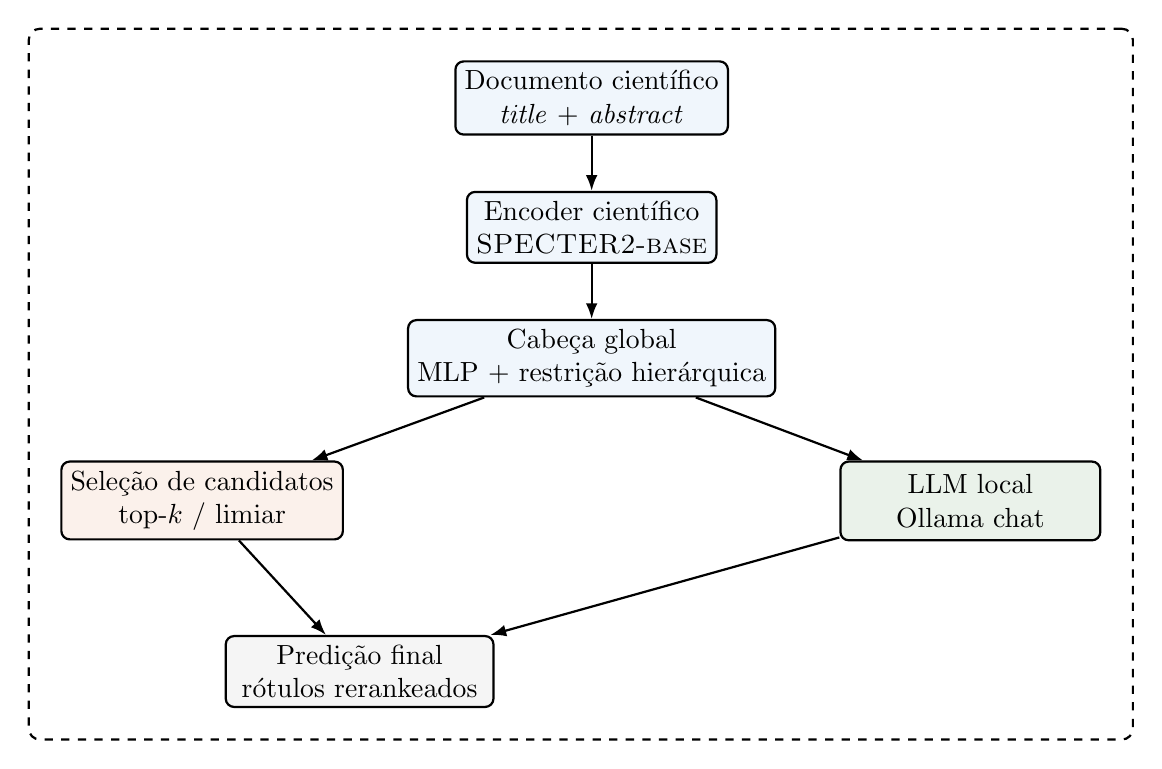
\begin{tikzpicture}[
  node distance=7mm and 12mm,
  box/.style={draw, rounded corners=3pt, thick, align=center, minimum height=9mm, minimum width=30mm, fill=ourblue!6},
  gate/.style={draw, rounded corners=3pt, thick, align=center, minimum height=9mm, minimum width=31mm, fill=ourorange!10},
  llm/.style={draw, rounded corners=3pt, thick, align=center, minimum height=10mm, minimum width=33mm, fill=ourgreen!10},
  outbox/.style={draw, rounded corners=3pt, thick, align=center, minimum height=9mm, minimum width=34mm, fill=gray!8},
  arrow/.style={-{Latex[length=2mm]}, thick}
]
\node[box] (doc) {Documento científico\\\textit{title} + \textit{abstract}};
\node[box, below=of doc] (enc) {Encoder científico\\\textsc{SPECTER2-base}};
\node[box, below=of enc] (clf) {Cabeça global\\MLP + restrição hierárquica};
\node[gate, below left=8mm and 8mm of clf] (filter) {Seleção de candidatos\\top-$k$ / limiar};
\node[llm, below right=8mm and 8mm of clf] (llm) {LLM local\\Ollama chat};
\node[outbox, below=12mm of filter, xshift=20mm] (final) {Predição final\\rótulos rerankeados};

\draw[arrow] (doc) -- (enc);
\draw[arrow] (enc) -- (clf);
\draw[arrow] (clf) -- (filter);
\draw[arrow] (clf) -- (llm);
\draw[arrow] (filter) -- (final);
\draw[arrow] (llm) -- (final);
\node[draw, dashed, rounded corners=4pt, thick, inner sep=4mm, fit=(doc)(enc)(clf)(filter)(llm)(final)] {};
\end{tikzpicture}
\end{center}
\end{document}
